\documentclass[12pt]{article}

\usepackage[utf8]{inputenc}
\usepackage{graphicx}
\usepackage{fancyhdr}

\title{g55\_7\_segment\_decoder - Display Input as Hexadecimal or Card Value}
\author{Group 55\\Juliette Regimbal (260657238)\\Qingzhou Yang (260687570)}
\date{February 20, 2017}
\pagenumbering{gobble}
\pagenumbering{arabic}
\pagestyle{fancy}

\begin{document}
\maketitle
\setlength{\parindent}{0ex}
\lhead{Group 55}
\rhead{Juliette Regimbal (260657238)\\Qingzhou Yang (260687570)}
\section{Circuit Description}
The \textit{g55\_7\_segment\_decoder} circuit takes a 4-bit input called code that stores an unsigned integer, and a 1-bit input called mode that sets if the output should be in hexadecimal (low) or if the number should be displayed as the equivalent card value in a standard deck (high). The output is a 7-bit active-low bus meant to be connected to a 7 segment display. Bit 0 goes to segment 0, bit 1 goes to segment 1, and so forth. Since the values in a deck of cards only goes up to 12 (a king), numbers greater in this will be displayed as a `-' in card mode. Since the number 10 exists in the card display, only the 0 is displayed.\\

The pinout for the circuit is as follows:
\begin{figure}[h!t]
\centering
	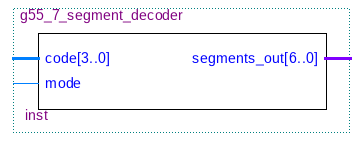
\includegraphics[scale=0.5]{graphics/7_seg_schematic.png}
	\caption{\textit{g55\_7\_segment\_decoder} Pinout}
\end{figure}

\section{Circuit Testing}
The \textit{g55\_7\_segment\_decoder} was tested for all possible inputs by combining the code and mode inputs into a signle 5-bit word that was set from $00000_2$ to $11111_2$. The output was recorded and verified by plotting it in ModelSim. The waveform out is as follows:
\begin{figure}[h!t]
\centering
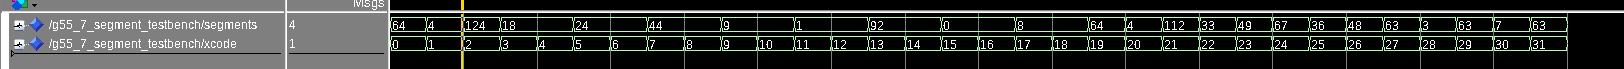
\includegraphics[scale=0.3]{graphics/7_seg_wave.png}
\caption{\textit{g55\_7\_segment\_decoder} Test Wave}
\end{figure}

\end{document}